\chapter{Extending the toolset}
\label{chp:extensibility}
\label{bkm:Extensibility}There are various mechanisms for enhancing or extending the functionality of \ProductName{}, which go beyond customisation
of the user interface. Some of these mechanisms are separate products with their own documentation. These are the `C' programmer's API
for Unix and the API for Windows PCs.

This chapter covers the facilities which are built into the basic product and the Motif GUI option as standard. They consist of hooks
where \ProductName{} can invoke custom built user, administrator and internal programs. Such programs are usually shell scripts, but compiled
programs can be used just as easily.

\section{Message Handling}
It is possible to ``intercept'' the message handling of job completion messages.

There are two kinds of job completion messages, as well as the automatic mailing of standard output and standard error to the user unless
redirected.

These are ``mail completion message'' and ``write completion message to terminal''.
The latter case may vary, depending upon whether the originating host was a Unix machine or a Windows client.

Standard action is to invoke the mail program for ``mail completion'', \progname{btwrite} to send
messages to the user's terminal if on a Unix machine and \progname{dosbtwrite} to send messages if on a Windows
client.

The actual messages which are sent are generated by the internal program \progname{btmdisp}, and this usually extracts the message
texts from the internal help file \filename{btint-config} in the system help directory \helpdir.

You can customise this in various ways:

\begin{enumerate}
\item You can customise the messages in the \filename{btint-config} file itself.
\item Various users can specify their own \filename{btint-config} file replacement.
\item Each of the 3 message sending programs can be reselected on a system-wide or individual basis.
\end{enumerate}
\subsection{Customising the system message file}
All of the various mail or ``write'' messages are grouped together. There are variations according to whether the job
terminating had an error or not, and a title or not.

Various \exampletext{\%t} etc parameters are inserted, the meaning should be reasonably clear from the context.

\subsection{Specifying a customised message file}
A user can specify a message file for his or her own use to replace the system message file, by including a line with the keyword
\filename{SYSMSG} in a \homeconfigpath{} file in his or her home directory. This takes the form

\begin{expara}

SYSMSG=alternative/file

\end{expara}

If this is not an absolute location (i.e. starting with ``\exampletext{/}''), then the
location will be relative to the home directory.

Only job completion messages need to be placed in the file designated thus. Only jobs owned by the user will use this file; other users will
receive a message from the system file or from their own message file if specified.

If the specified file cannot be opened, then the system message file is reverted to.

\subsection{Specifying alternative job completion - system wide}
The three job completion programs, the mail program, \progname{btwrite} and \progname{dosbtwrite}
may be respecified by assignment to the environment variables \filename{MAILER}, \filename{WRITER} and
\filename{DOSWRITER} within the master configuration file, \masterconfig.

The replacements may be shell scripts rather than programs.

Remember to use the ``\exampletext{:}'' notation rather than ``\exampletext{=}'' unless you
want these assignments to be passed to Batch jobs.

For example:

\begin{expara}

MAILER:/usr/local/bin/my-batch-mailer

\end{expara}

Each program is passed a user name as an argument, and a message on standard input derived from the message file.

A simple replacement mailer shell script \filename{/usr/local/bin/my-batch-mailer} in the above example might be as follows:

\begin{expara}

\#! /bin/sh

\bigskip

(echo To: \$1;cat)|/usr/sbin/sendmail -t

\end{expara}

Them main function of this would be to properly format the mail headers with a subject line.

\subsection{Specifying alternative job completion programs - per user}
Alternative message programs may be specified by assignments to \filename{MAILER}, \filename{WRITER} and
\filename{DOSWRITER} within a user's \homeconfigpath{} file off his or her home directory.

Thus:

\begin{expara}

WRITER=/my/write/program

\end{expara}

Note that the ``\exampletext{:}'' notation is not recognised here.

If the program does not exist or fails, the message is silently lost.

All programs are run completely under the identity of the job owner.

\section{Command Interpreters}
By default, new \ProductName{} installations have just one command interpreter set up, usually the Bourne shell.
Additional command interpreters can be added. These can use the same shell programs as existing command
interpreters, but with different parameters or just different names.
The parameters include arguments, like \exampletext{{}-s},
passed on the shell command line, nice values and \ProductName{} load levels.

As well as the Bourne, Korn and ``C'' shells, any program which reads its commands from standard input may be set up
as a command interpreter, such as \progname{perl} and various SQL programs.

Some databases have command interpreters which will read their commands from standard input. The normal approach would be to write a shell
script that invokes the database command interpreter with the name of a command file. If the command interpreter will read from standard input
the ``shell script wrapper'' can be dispensed with.

Bespoke command interpreters can also be written. These can be compiled programs or shell scripts.

For example, a command interpreter could be written to \exampletext{bypass} or \exampletext{dummy\_run}
jobs. That is run the job but not execute any of the commands inside. The effect being to make it appear to the rest of the system as though
the job ran and finished normally. This could be used for testing schedules of jobs at a simple level without doing any processing.

A shell script for such a command interpreter might look like this:

\begin{expara}

\#!/bin/sh

\bigskip


echo Job bypassed

exit 0

\end{expara}

Such a script could be expanded to check for job control variable operations that could invalidate testing a job schedule in this manner.

\section{Custom Tools \& Scripts}
The command line programs for \ProductName{} enable all job, variable, user and general information to be queried and / or modified.
These can be built into new commands using shell scripts or used within user applications. Here are some ideas.

\subsection{Custom Tools}
A user may have an application which queries and performs updates on a database. Some of the activities, like handling telephone enquiries,
obviously require immediate processing. Many tasks, such as changing a customers details and producing long reports, can be performed in the
background or overnight.

The application could submit batch jobs to performs these activities, and query \ProductName{} to find out how such jobs are progressing.

The actions that could be performed include:

\begin{itemize}
\item Getting a list of the batch jobs (submitted to run once and be retained) that have worked for a particular user or set of users. The
application would use a command like:

\begin{expara}

\BtjlistName{} -u \$USER -F {\textquotedbl}\%h \%P\#{\textquotedbl} {\textbar}
grep {\textquotedbl}Done{\textquotedbl}

\end{expara}

The option \exampletext{{}-u \$USER} restricts the display to the current user and the \exampletext{{}-F}
``string'' option formats the output to contain just the title and progress fields. The output will look like
this:

\begin{expara}

prog\_a \ \ \ \ \ \ \ \ Done

Tuesday\_backup Done

update \ \ \ \ \ \ \ \ Done

\end{expara}

\item Submitting batch jobs to run after a specified time. The assignments and pre-conditions can also be used to handle other
dependencies, such as

\begin{enumerate}
\item Ensuring all database update jobs are completed before starting any query or report jobs.
\item Stopping the back up jobs from starting until all others are done.
\item The database access is likely to deteriorate if too many processes are accessing it at once. The variables can be used as semaphores to
make sure the optimum number of jobs are using the database at any time.
\end{enumerate}
\item The \PrBtq{} and \PrXmbtq{} tools can also be invoked from inside an application. So the application could invoke the
tool with a restriction to show those jobs of relevance to the current part of the application being used.
\end{itemize}
\subsection{Shell Scripts}
An infinite variety of useful commands can be created using shell scripts. The activities described in the previous sub-section can just
as easily be performed by stand alone shell scripts. Other simple examples include:

\begin{itemize}
\item Cancelling all batch jobs that match a certain criteria. For example test jobs may be in a queue called junk. If the script takes
the queue name as an argument the command might be:

\begin{expara}

canjobs junk

\end{expara}

and the script would be

\begin{expara}

\BtjlistName{} -q \$1 -F {\textquotedbl}\%N{\textquotedbl} {\textbar} while read JOB

do

\ \ \ \ \BtjchangeName{} -C \$JOB

done

\end{expara}

This fragment of shell script could be written in a variety of ways, some of which would only take up one line. The form used above was
chosen for clarity, rather than as a style guide. \item Viewing the output from a job which has stdout redirected to a
file. If the script takes the job number as an argument the command might be:

\begin{expara}

viewlog \textit{jobno}

\end{expara}

and the script might be

\begin{exparasmall}

\# Get the list of I/O redirections for the job.

\# Use tr to Separate each redirection out - one per line.

\# Pipe into sed to substitute the job id number for any

\# \%d1 symbols in the path/file names. Then pipe into awk

\# to get the stdout filename.

\bigskip


\BtjlistName{} -F {\textquotedbl}\%R{\textquotedbl} \$1 {\textbar} {\textbackslash}

tr {\textquotedbl},{\textquotedbl} {\textquotedbl}{\textbackslash}n{\textquotedbl} {\textbar} {\textbackslash}

sed s/\%d1/\$1/g {\textbar} {\textbackslash}

awk -F{\textquotedbl}{\textgreater}{\textquotedbl} {\textquotesingle} ! /\^{}2/

\&\& ! /0/ \{ print \$NF \} {\textquotesingle} {\textbackslash}

read OUTFILE

\bigskip


\# \ If the stdout file exists then open it for viewing

\# \ in using view, the read only version of vi.

\bigskip

if [ -f {\textquotedbl}\$OUFTILE{\textquotedbl} ]

then

\ \ \ \ \ \ view \$OUTFILE

fi

\end{exparasmall}

This is a cut down version of an actual script used on an X-Terminal which opened a separate window for \exampletext{stdout} and
\exampletext{stderr}. If the job was running, the script ran the \exampletext{tail -f} command in a terminal session or the
\progname{vi} editor if the job had finished. As a further refinement the background colour of the terminal session was set to
reflect the jobs state - green = done, yellow = running and red = failed.
\end{itemize}
Useful shell scripts can usually be adapted to be run as macros from within \PrBtq{}, \PrXmbtq{},
\PrBtuser{} and \PrXmbtuser{}. In the case of \PrBtq{} and \PrXmbtq{} they have to be modified to take a job number or variable name as their
only argument from the command line. User administration macros can take a list of user names as their arguments.

To run the output file viewer the shell script may be used exactly as it is.

The example to cancel jobs in a particular queue can be modified to become a macro. A line must be added at the beginning to query the
selected job, using \PrBtjlist{} with the job number, to get the queue name. The result should look like:

\begin{exparasmall}

Q\_NAME={\textasciigrave}\BtjlistName{} -F {\textquotedbl}\%q{\textquotedbl} \$1{\textasciigrave}

\BtjlistName{} -q \$Q\_NAME -F {\textquotedbl}\%N{\textquotedbl} {\textbar} while read JOB

do

\ \ \ \ \ \BtjchangeName{} -C \$JOB

done

\end{exparasmall}

Once set up the user would run the macro, from within \PrBtq{} or \PrXmbtq{}, by selecting any one of the jobs in the required queue and then invoking
the macro.

\section{Macros for Interactive User Programs}
\label{bkm:Macrodefs}Macro command facilities are incorporated in the commands \PrBtq{}, \PrBtuser{}, \PrXmbtq{} and \PrXmbtuser{}.

Up to 9 pre-defined macro commands can be set up for jobs and another 9 for variables in \PrBtq{} and \PrXmbtq{}. Similarly up to 9 pre-defined macro
commands can be defined for users in \PrBtuser{} and \PrXmbtuser{}. In addition all of these programs can run macros which are not pre-defined. In this case the programs prompt for the name of the macro to run.

The macro does not have to be anything to do with the context of jobs, variables or users. It will, however, always be passed the identity of
the currently-selected item or user as a parameter or parameters.

The actual commands are placed in the relevant help files, which by default are \filename{btq.help},
\filename{xmbtq.help}, \filename{btuser.help} and \filename{xmbtuser.help} in \filename{/usr/spool/progs}. For the Motif programs, the names
on the menu options are specified in the resource file.

\subsection{Inserting the commands}
First specify the macro commands in the help file as follows:

\begin{expara}

27000P:Prompt for prompted command

27001P:cmd1

27002P:cmd2

27003P:cmd3

27010P:Prompt for prompted command

27011P:cmd1

27012P:cmd2

\end{expara}

The \exampletext{2700nP} prompts specify the pre-defined macros, where n is in the range 1 to 9, for jobs in \PrBtq{}, \PrXmbtq{} and users in
\PrBtuser{}, \PrXmbtuser{}. The 27000P entry specifies the prompt used for job / user macros which are not pre-defined.

Pre-defined Macros for variables are specified by prompts of the form \exampletext{2701nP}, where \textit{n} is in the range 1 to 9.
The \exampletext{27010P} entry specifies the prompt used for variable macros which are not pre-defined.

The command involved is any arbitrary shell command which may take a jobs, variables or list of users as the case may be. (The command may
be given zero users by \PrXmbtuser{} and \PrBtuser{} if none are selected).

\PrBtq{} and \PrBtuser{} assume that all macro commands run silently without producing any output on the screen or interacting with the user. If a macro needs access to the screen and or keyboard, put an exclamation mark immediately following the colon in the specification. For example:

\begin{expara}

27001P:!cmd1

\end{expara}

This will instruct \PrBtq{} or \PrBtuser{} to redraw the screen after completion.

\subsection{Menu Options in the Motif Programs}
Menu options are automatically created in \PrXmbtq{} and \PrXmbtuser{}. The names given to the options can
be set by editing the relevant lines in the resource file. The menu options for job macros in \PrXmbtq{} are specified in
lines of the form:

\begin{expara}

\XmbtqName*jobmacro*macro1.labelString: \textit{option text}

\end{expara}

Here \exampletext{macro1} indicates that this is the definition for the first option in the jobmacro menu. It will run macro 1 as set
up by the prompt definition for \exampletext{27001P:} in the \exampletext{xmbtq.help} message file. The option text
specifies the text to appear in the menu for that option.

For example, the following lines:

\begin{expara}

\XmbtqName*jobmacro*macro1.labelString: View job output

\XmbtqName*jobmacro*macro2.labelString: Delete job output

\end{expara}

will produce a menu looking like this

 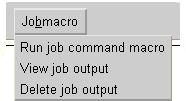
\includegraphics[width=4.867cm,height=2.671cm]{img/ref54.jpg} 

The equivalent lines for specifying variable macros in \PrXmbtq{} and user macros in \PrXmbtuser{} are respectively:

\begin{expara}

\XmbtqName*varmacro*macro1.labelString:

\XmbtuserName*menubar*macro1.labelString:

\end{expara}

The resource files used by Motif are not quite as flexible in scope as the \ProductName{} message files. Copies of the \filename{XI} file
(holding \ProductName{} resources) can probably only be set up globally and one alternative for each user in their home directory. The lines shown
above can be tailored on invoking \PrXmbtq{} or \PrXmbtuser{} using the \exampletext{{}-xrm} option.

\subsection{Binding the keys in \BtqName{} and \BtuserName}
To use macros in \PrBtq{} and \PrBtuser{} it is necessary to specify what key to press to invoke the macro. This is often called binding the keys.

To bind the keys, assign key codes 600 to 609 in the relevant message file. For example:

\begin{expara}

K600:0

K601:{\textbackslash}kF1

\end{expara}

will assign the ``0'' key to the prompted-for command and F1 to the first ``pre-defined'' command. In \PrBtq{} this will assign the same key to
the first ``pre-defined'' command for both the variable and job macros.

To assign different keys for job and variable macros, use the state keys by prefixing with the relevant state number. This is 1 for the job
screen and 2 for the variable screen. For example to define five job macros and one variable macro using consecutive function keys:

\begin{expara}

1K601:{\textbackslash}kF1

1K602:{\textbackslash}kF2

1K603:{\textbackslash}kF3

1K604:{\textbackslash}kF4

1K605:{\textbackslash}kF5

\bigskip

2K601:{\textbackslash}kF6

\end{expara}

\subsection{Example - Adding the ``cancel all jobs in queue'' to \BtqName}
The shell script, described earlier, for cancelling all the jobs in a particular queue is an ideal candidate for a macro. To recap, the shell
script is called \exampletext{canjobs} and it contains the these commands:

\begin{exparasmall}

Q\_NAME={\textasciigrave}\BtjlistName{} -F {\textquotedbl}\%q{\textquotedbl} \$1{\textasciigrave}

\BtjlistName{} -q \$Q\_NAME -F {\textquotedbl}\%N{\textquotedbl} {\textbar} while read JOB

do

\ \ \ \ \ \ \BtjchangeName{} -C \$JOB

done

\end{exparasmall}

Cancelling a job is normally assigned to lower case \exampletext{z}, so it might be helpful if cancelling all jobs
in a queue is assigned to upper case \exampletext{Z}. This command should also be added to the help message for the job screen.
The following extracts show the changes and additions, in bold type, to the \BtqName{} message file. The dotted lines indicate omitted lines of text.

\begin{exparasmall}

\ \ \ \ \ \ \ ............

\# Keys for displaying job list

\bigskip


H1:? \ \ \ \ \ \ \ \ \ \ \ Help (this screen)

\ \ \ \ \ \ \ ...

H1:P \ \ \ \ \ \ \ \ \ \ \ Reset progress code

H1:r z \textbf{Z} \ \ \ \ \ \ \ Set runnable, cancelled \textbf{, all in queue cancelled}

H1:g f \ \ \ \ \ \ \ \ \ Run if possible ignoring time adv time/no adv time

\ \ \ \ \ \ \ ...

1K523:r

1K524:z \ \ \ \ \ \ \ \ \textit{(this is the key assignment for set cancelled)}

\ \ \ \ \ \ \ ...

1K532:a

1K540:{\textbackslash},

\bigskip


1k601:{\textbackslash}KF1

\textbf{1K602:Z} \ \ \ \ \ \ \ \ \textit{(this is the key assignment for the new macro)}

\ \ \ \ \ \ \ ............

\bigskip


\# Example macro commands

\# Jobs are 27000 + n, variables 27100 + n n is 0 to 9, 0 prompts

\bigskip


27000P:Run what:

H27000:Please give the command you want to run.

H27000:The job number will be given as a parameter.

27001P:!viewlog

27002P:canjobs

27100P:Run what:

H27100:Please give the command you want to run.

H27100:The variable name will be given as a parameter.

\end{exparasmall}

The first macro defined in the prompts is the viewlog script described earlier. It is obviously an interactive macro, hence has the
exclamation mark ``\exampletext{!}''after the colon ``\exampletext{:}'' to tell \BtqName{} to release the screen and redraw it afterwards.

\section{File \& Event Monitoring}
Note: This section is largely superseded by the introduction of \PrBtfilemon{}, but is left in as an example of how
various operations may be done.

An event can be detected by polling for a change in state of the object affected by the event. For a batch processing schedule, the most likely
events of interest are file creation, modification or deletion. Two of the benefits of polling for a specific event, rather than intercepting
all events, are:

\begin{enumerate}
\item Machine resources are only used for the events of interest. E.g. only the relevant file or files are being checked.
\item An event need only be polled for when it is of interest. E.g. a job may need a particular file as a pre-requisite, but there is no
point polling for the file until the job's scheduled run time.
\end{enumerate}
Two suggestions follow, for file monitoring, which can be adapted to any event which can be tested for by some change in state.

\subsection{Polling for Arrival of a File}
A simple shell script can be used to look for a file arriving, then setting a job control variable and exiting when it is found. There are
4 parameters that can be specified from the command line to provide a general purpose script. They are: filename
(\exampletext{\$1}), time interval between tests
(\exampletext{\$2}), variable name
(\exampletext{\$3}) and value to write into variable
(\exampletext{\$4}).

\begin{expara}

\#!/bin/sh

\# This example tests for a file \$1 existing

\# every \$2 seconds. When the file is found it

\# sets the contents of variable \$3 to be the

\# value \$4.

\bigskip


while [ ! -f \$1 ]

do

\ \ \ \ sleep \$2

done

\bigskip


\BtvarName{} -s \$4 \$3

\end{expara}

\subsection{Continuous Polling for a constantly changing list of Files}
If a large number of files are being monitored then it is probably more efficient to have one process doing the polling. The list of files
could be specified in a file loaded by the file monitor program when it starts. This would mean however that the program had to be restarted
whenever the list of files changes.

The job control variables can be used to hold the list of files to poll for as well as returning the
status. In this example the variables conform to this set of conventions:

\begin{itemize}
\item Names of variables involved in file monitoring all end with the string \exampletext{\_FILE}, for example
\exampletext{UserAdmin\_FILE}, \exampletext{customer\_FILE}.
\item The comment field must contain the full path and name of the file to look for.
\item Variables must contain the value ``\exampletext{Waiting}'' when the file they represent is to be polled for.
\item The value of variables will be set to ``\exampletext{Ready}'' when their file has been detected.
\end{itemize}
The script looks like this:

\begin{exparasmall}

\#!/bin/sh

\bigskip


while :

do

\ \ \ \ \BtvlistName{} -F {\textquotedbl}\%N \%V \%C{\textquotedbl} {\textbar} grep {\textquotesingle}\_FILE\${\textquotesingle} {\textbar}{\textbackslash}

\ \ \ \ while read NAME VALUE COMMENT

\ \ \ \ do

\ \ \ \ \ \ \ \ if [ {\textquotedbl}\$VALUE{\textquotedbl}={\textquotedbl}Waiting{\textquotedbl} ]

\ \ \ \ \ \ \ \ then

\ \ \ \ \ \ \ \ \ \ \ \ if [ -r \$COMMENT ]

\ \ \ \ \ \ \ \ \ \ \ \ then

\ \ \ \ \ \ \ \ \ \ \ \ \ \ \ \ \BtvarName{} -s {\textquotedbl}Ready{\textquotedbl} \$NAME

\ \ \ \ \ \ \ \ \ \ \ \ fi

\ \ \ \ \ \ \ \ fi

\ \ \ \ done

\ \ \ \ sleep 120

done

\end{exparasmall}

Parameters which are hardwired into this example, like the number of seconds for the sleep command, could be supplied as arguments to the
script file monitoring.

